\documentclass{beamer}
\usepackage[T1]{fontenc}
\usepackage[utf8]{inputenc}
\usepackage{lmodern}
\usepackage[brazil]{babel}
\usepackage{graphicx}
\usepackage{caption}
\usepackage{subcaption}

\captionsetup{compatibility=false}

\usetheme{JuanLesPins}
\useoutertheme[subsection=false]{miniframes}

\setbeamertemplate{frametitle}[default][center]
\title{
       \textbf{Mezuro} \\
      }
\subtitle{
		\textbf{CCSL - IME - USP}
		}
\author{Diego Araújo\\
        Rafael Manzo
       }

\begin{document}

\maketitle

\section{Introdução}

\begin{frame}
  \frametitle{A história do projeto}
  \framesubtitle{}

  \begin{itemize}
    \item Nasceu no Instituto de Matemática e Estatística como projeto de doutorado do atual professor da UNB Paulo Meirelles
      \begin{itemize}
        \item Primeira aparição em XP ainda em 2009 como Kalibro
      \end{itemize}
    \item Teve como forte colaborador o atual mestre Carlos Morais através do projeto Kalibro
    \item É apoiado e mantido pelo Centro de Competência em Software Livre(IME/USP) e financiado pelo Napsol
    \item Atualmente conta com a colaboração de alunos do IME/USP

  \end{itemize}

\end{frame}

\section{Motivação}
\begin{frame}

  \frametitle{Métricas de Software}
  \begin{center}
  You cannot control what you cannot measure.\footnote{Tom DeMarco. Controlling software projects. management, measurement and estimation. ISBN, 10(0131717111):0–13.}
  \end{center}


\end{frame}


\begin{frame}
  \frametitle{Métricas de software}
  \framesubtitle{Problemas atuais}

  \begin{itemize}
    \item Não há parâmetros de comparação consolidados
    \item Existem estudos, mas poucos dados empíricos
    \item Ainda é dada pouca importância ao monitoramento de código
  \end{itemize}
\end{frame}

\begin{frame}
\frametitle{Exemplos de métricas de software}


  \begin{figure}
        \begin{subfigure}[b]{0.3\textwidth}
      \includegraphics[width=\textwidth]{images/size.png}
                \caption*{Tamanho das entidades}

        \end{subfigure}\qquad\qquad\qquad\qquad\qquad%
        ~ %add desired spacing between images, e. g. ~, \quad, \qquad etc.
          %(or a blank line to force the subfigure onto a new line)
        \begin{subfigure}[b]{0.3\textwidth}
      \includegraphics[width=\textwidth]{images/cohesion.png}
                \caption*{Nível de responsabilidade (coesão)}
        \end{subfigure}
        \begin{subfigure}[b]{0.3\textwidth}

      \includegraphics[width=\textwidth]{images/coupling.png}
                \caption*{Acoplamento}

        \end{subfigure}
        \caption{Métricas de software}\label{fig:animals}
\end{figure}

\end{frame}

\section{Solução}

\begin{frame}
  \frametitle{Proposta}
  \framesubtitle{}

  Encontrar conjuntos de métricas e interpretações, mantendo sua evolução no tempo, de acordo com situações específicas, através de:
  \begin{itemize}
    \item Ferramentas base para coleta das métricas\footnote{Analizo, Checkstyle, CVSAnaly etc.}
    \item Gerenciador de configurações e análise do resultado da coleta\footnote{Kalibro}
    \item Interface web para interação com a comunidade\footnote{Mezuro}
  \end{itemize}


\end{frame}
  \section{Mezuro}
  \begin{frame}
    \frametitle{Mezuro}
    \framesubtitle{O que é?}

    \begin{figure}
      \begin{flushleft}
      \begin{center}
      \includegraphics[width=4.3cm, height=1.4cm]{images/logo-mezuro.png}
      \end{center}

        \label{fig:logo-mezuro}
      \end{flushleft}
    \end{figure}

    \begin{itemize}
      \item Rede social para desenvolvedores de software
      \item Permite compartilhar metodologias de avaliação do código de softwares, bem como seus resultados
      \item Visualização fácil dos resultados da análise e criação de novas configurações de métricas para a comunidade
    \end{itemize}

  \end{frame}

  \subsubsection{Demonstração}
    \begin{frame}
      \frametitle{Página inicial}

      \begin{figure}
        \begin{center}
          \includegraphics[width=11cm, height=6cm]{images/main.png}
          \label{fig:home}
        \end{center}
      \end{figure}

    \end{frame}

    \begin{frame}
      \frametitle{Exemplo de processamento}
      \framesubtitle{CyanogenMod}

      \begin{figure}
        \begin{center}
          \includegraphics[width=11cm, height=6cm]{images/cyano.png}
          \label{fig:home}
        \end{center}
      \end{figure}
    \end{frame}

  \section{Contexto}
    \begin{frame}
      \frametitle{Cliente}
      \framesubtitle{Nós}

      \begin{center}
        \textbf{Os anciões}
        \begin{columns}[c] % the "c" option specifies center vertical alignment
          \column{.33\textwidth} % column designated by a command
           \begin{figure}
              \begin{center}
                
\includegraphics[height=.5\textheight]{images/manzo.jpg}
                \caption{Manzo}
              \end{center}
            \end{figure}
          \column{.33\textwidth}
           \begin{figure}
              \begin{center}
                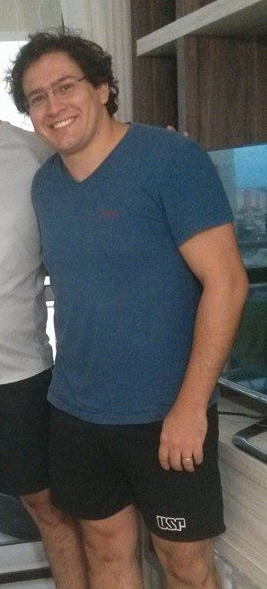
\includegraphics[height=.5\textheight]{images/paulo.png}
                \caption{Paulo}
              \end{center}
            \end{figure}
          \column{.33\textwidth}
           \begin{figure}
              \begin{center}
                
\includegraphics[height=.5\textheight]{images/diego.jpg}
                \caption{Diego}
              \end{center}
            \end{figure}
        \end{columns}
      \end{center}
    \end{frame}

    \begin{frame}
      \frametitle{Cliente}
      \framesubtitle{Dilma}

      \begin{figure}
        \begin{center}
          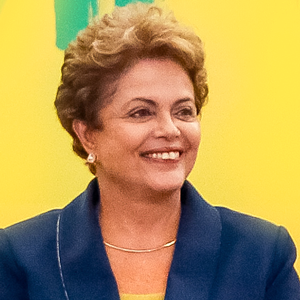
\includegraphics[height=.5\textheight]{images/delma.png}
          \caption{Novo Portal do Software Público Brasileiro}
        \end{center}
      \end{figure}
    \end{frame}

  \section{Conclusão}
    \begin{frame}
      \frametitle{O quê esperar deste projeto}
      \framesubtitle{}

      \begin{itemize}
        \item Interagir com outras equipes
        \item Muito código
          \begin{itemize}
            \item Modularizado
            \item Qualidade
            \item Totalmente reescrito recentemente
            \item 100\% em Ruby
          \end{itemize}
        \item Ambiente de simples configuração
        \item Software em produção
        \item Muitas práticas ágeis
      \end{itemize}
    \end{frame}

    \begin{frame}
      \frametitle{Onde nos encontrar}
      \framesubtitle{}
      \begin{center}
      Projeto: \\ \url{http://mezuro.org}
      \\~\\ Repositório de códigos: \\ \url{https://github.com/mezuro}
      \end{center}
    \end{frame}

\end{document}
